\documentclass{article}
\usepackage[utf8]{inputenc}

\title{Lecture 5: topic beyong sigfigence}
\author{wbg231 }
\date{November 2022}
\usepackage{tikz,graphicx,amsmath,amsfonts,amscd,amssymb,bm,cite,epsfig,epsf,url}
\begin{document}

\maketitle

\section{P values}
\subsection{cult of the p-value}
\begin{itemize}
%\item 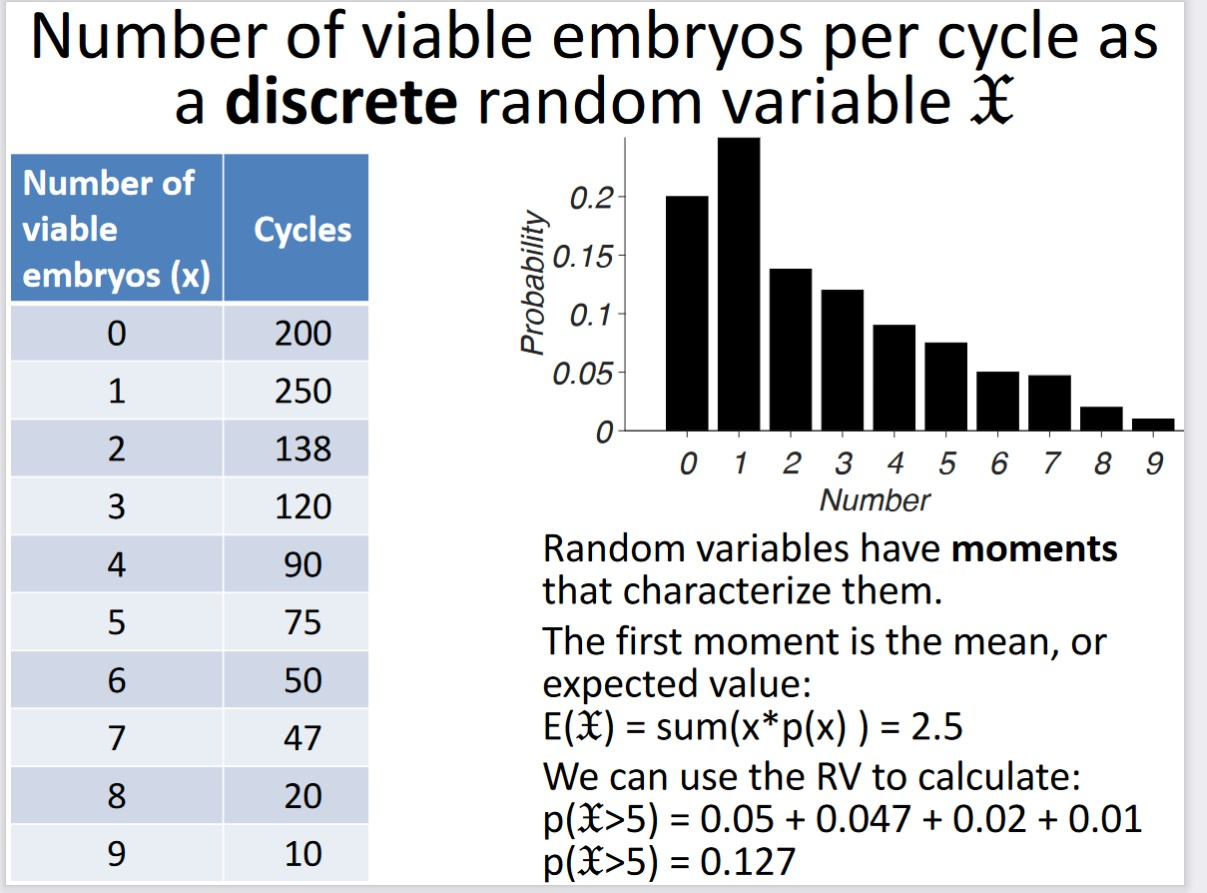
\includegraphics[width=7.5cm]{Final_Review/Lecture_2/lecture_1example.jpg}
\item science is based all around significance it is all about getting significant results
\item science is the cult of senescence
\item about 97\% of papers have a p value that is significant 
\item science has a preference for significant results 
\item significant needs to be backed up by 3 things
\begin{enumerate}
    \item effect size 
    \item statistical power
    \item confidence 
\end{enumerate}
\section{ p hacking }
\item there is a replicability crisis, because many p values can not be replicated.
\item in the 2000s, there were a lot genomics that founded if you have  certain stick of this allele that is related to serotonin you are more likely to be depressed 400 pa pres were published.
\item  they were all false positives the replication rate in this field is literally 0.
\subsection{signs are everywhere}
\item if we plot the distribution of p values in papers. there are a huge amount around .4 
\item there is a bimodal distribution one peak close to zero and another that is very close to 5. p values a random viable that is a beta distribution. if the beta is null is false the distribution of p value should be uni modal and have a peak near 0. 
\item  if the null is true the p value u should be zero one distribute uniform so there should be 5\% false positives if there is no bias
\item the second peak is likely coming from the scientists. 
\subsection{how is this possible}
\item $\alpha=.05$ sets the false positive error at 5\% for a single test
\item there are systematic cultural reasons, scientists are incentives 
\item there are proximal causes, ie the researcher has many ways to get a certain p value, that is p hacking. ie teh scientists have some flex ability when analyzing 
\item the root causes is a lack of statically power. 
\subsection{proposed issue}
    \item a true positive or false positive are the only good outcome for scientists
    \item there are more false positives published than true positives. 
    \item if the root cause is that scientists have to much flammability to change the analysis, we should have them pre-register what analysis they plan to do prior to starting there study. 
    \item pre registration ahs a good effect on the colture 
    \item this only fixed the proximal cause
    \item it is hard to do data anlysis before you start to wrok with it, so it can be very limitiing 
    \itme also people could just not follow there pre registation idea
\subsection{effect size :coehn's d}
\item reaserch chould be about finding effect size 
\item suppose we are testing if the a drug increases iq. we test it on 20,000 poeple and find sttitically sigfngat results 
\item but at that level of n something like a .05 iq incrase is not relvent 
\item so staticial sigfgance is nto the same as pracitcal sigfgence 
\item coehns d is $\frac{\mu_1-mu_2}{}\sigma$ so it is the difference between the two population means devided by there joint statnadrd deviation 
\item Cohen's d normalzied the mean difrence by the standard devation not the standard error
\item the $SEM=\frac{\sigma}{\sqrt{n}}$ so at sample size of 1 $SEM=\sigma$
\item so this has an implied sample size of 1, how much does this matter for the indivudal 
\item teh sameller th emean difrence the smaller the effect size
\item this is a way to standardize the relative mean difference
\item cohns s is for comparing 2 means it is a good effect size metric 
\item effect size also allows us to compare significance across studies 
\item when ever you see a big varition in the effect size then we think that the study was liekly under powered. 
\itme cohens d does not deppend on sample size os we can compare effects
\subsection{how big should sample size be}
\item if we are looking for a big effect, the sample size does not need to be large 
\item if we are looking for very subtle effects, we need a large sample size
\item if cohns mean is 8 there is no overlap so just need 1 of each sample
\item think nba players and pigmies
\item effect deals with population 
\item male female high diference is 2d use that as scale for effect
\item the whole point of data science is about finding small effects
\item how large doe s a smaple size need to be to determine a diference between groups 
\itme d=1, n=20 (per group) looking at the graph it looks like they would be diferent 
\item 20 is resomable numebr for an effect size of 1. 
\item the typical effect size is $d=.25$ that means we need a larger n to reliably capture difference in sample means
\subsection{ statistical power}
\item when is enough enough 
\itme power is $power=1-\Beta$
\item this is related to our type 2 error rate, or our $\beta $ error 
\item statistical power is the probability of getting a significant result given the effect is real
\subsection{example of why this matters}
\item 1940's japan were waging war in the pecfic 
\item as the eruopene was distracted with teh eruopeene theater japan wanted to take oil in the picfic, but the isuse is the us naval fleet was there, so they did pearl harbor 
\itme but they missed three naval carriers that the us had 
\item by late may 1942 there were a number of boats that jaan had, they wanted to sue them to sync the us batter carriers
\item so the japanese forces were aproaching mid way 
\item immagine it is june 4th 1942, apraoching mid way. the question on his mind is do we do a strike midway or look first
\item we look firs tbecuase if we they stirke they get seen and could get lost 
\itme so they sent out 7 plaint over 176,000 miles. tha tis not a very carefull search that is 1 plain for half of england 
\item the japanese search plains did not find any charicters the genral intreperted that as the lack of finding carriers as evedince that there were no carriers
\item there were however carriers that the search pains missed
\itme so what power does is distinguish evedince of absance from evedince of absance 
\item so long story short the japanes enavy missed this war ship and then lost the batte
\subsection{back to power }
\item power is teh liklyhood of dettectign an effect if it is there
\item if there is to much sampleing error you may miss the effect even if it is there 
\item for a a score our test stat is $z=\frac{\bar(x)-\mu}{\frac{\sigma}{\sqrt{n}}-1}$
\item we can not change the numerator that is waht we are looking for 
\item the standard devation is also not under our control 
\item all that we can contorl is n ie the sample size in this example that would be the number of search plains 
\subsection{calcuatlint power }
\item in reality calcualtingf power is tough 
\item lower alpha leads to lower poiwer 
\item larger sampel size leads to larger power 
\item larger effect size leads to larger power
\item the type of test we chose to do also matters a lot pamatmeric tests are more powerufll than non-parmaetric tests
\item so we can just simulate power in practice.
\item in practice we really just estiamte teh power
\item \item 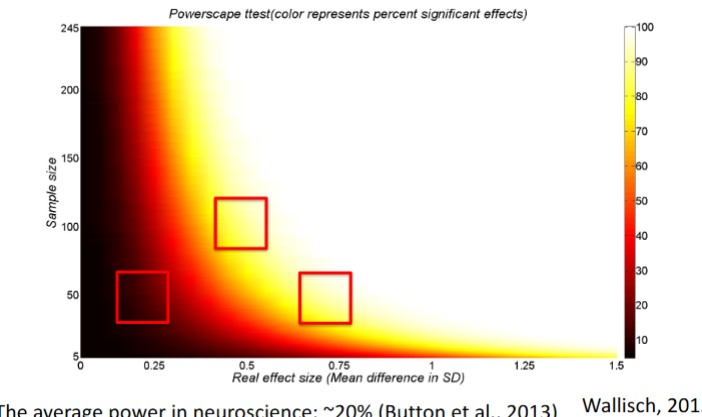
\includegraphics[width=7.5cm]{Final_Review/lecture_5/power scale .jpg} 
\item here we are shwoign the relaitonship of effect size and t tests.
\item we want to aim to be on the yellow curve adn have a target power of like .8
\item so like if the effect is real we want an 80\% cahnce of finding 
\item if there is a really large effect sizew we dont ened a huge n
\item but if the power is really low, you would expect to see only around 20\% of signifgant reulsts being published, but that is not the case this is back to replication issues.
\item the most effeicnet way to improve poer is to do study large effect szies
\item we can also try to have big data 
\subsection{the replicability crisis}
\item the replicability crisis is pretty much an issue of power
\item power also incrases square root of sample size
\item the root causes for p hacking is power
\item big data means that we have really large n and we thus have a lot of power, so we hopefully dont have to p hack. 
\item only a priori power is real power not post hoc power
\item the sample size demmands for power go up expontatially 
\subsection{big data primer}
\item big data allows us to distinguish tiny effects that are real from fake effects.
\item facebook found an effect size of 0.001 but they could find it becase they had a massive sample size
\item big data lets you find tiny effects, that may be omportat
\subsection{a priort power}
\item only a priori power is real power
\item post hoc or observed power is where youc alcuate the observed poer for the difrence in the empirical sample means 
\item but doing this could be problamatic becuse underpowerd samples vary a lot 
\item sampleing error can effect our esimate of the effect size
\item SSRI drugs could be much less effective than what we were led to bellive. 
\item instead we need to do a prior power 
\item the confidince intervals captures the wspread of our effect size, and the power shrinks the effect size. 
\item there is more to understnnd than just p values. 
\item that will make to a better science. 
\subsection{ confidence intervals }
\item lets say you show something is a significant effect, but given that we know there is an effect what margin or scale does that effect have. 
\item confidence intervals can help us understand a range of possible outcomes
\item the confdiince intervals is a range of plausbale values, so we want them as narrow as possible 
\item confidence intervals tie toghter effect, sigfence power, and sample size 
\item the p value quantifies sampling error  
\item the effect size was a statement about populaiton it is confidince intervals that let us understand the effecy size 
\item confdince intervlais an interval esiamte of the population parameter from the sampel
\subsection{whaat can confidince intervlas tell us?}
\item it depends who you ask 
\item some poepl say that it will tell you an esaimte of the likely siee of teh effect if there is an effect. 
\subsection{ confidicne intervals the calssical view}
\item this comes form pooling like for elletions 
\item the idea is that say we do our study and compute form our p-value teh 95\% confdiince interval from the study.
\item tehn we argue that the truee vlaue of the poualtin parmeter lies within the range of our cofidince interval 95\% of the time if we were to repeate our experimetn many times
\item so if we did this studymany time sthis tinervla would contina the ture value 95\% of the time, but we only do this once so the popualtion parameter is either in there or not 
\item any given sample ocnfdicne interval eithe rdoe sor doe snot caotinain the ture population parameter 
\item that is why it is called confidence not probability 
\subsection{calcuatioin }
\item the ise is to multiply a crtical z vlaue with the SEM. $SEM=\frac{\Sigma}{\sqrt{n}}$
\item crticial z vlaue found by taking the confdiince level and looking it up in the z table
\item so $ci=[\Bar{x}-Z_{\alpha/2}SEM]$ where our critical z vlaue is tetermined by our alpha level 
\item so the width fo teh interval increases as our alpha value goes up.
\item if we want to narrow the interval and make confdiicne bigger then we need to icnrease sample size 
\item suppose we fix n=10, as alpha goes up oru interval gets wider
\item suppose we fix alpha at some level we need to increase n  by more to narrow the smaple size
\item sample size is proportaional to sqrt of n 
\item CI give us more informaiton than siggence 
\item it allows us to distinguish absance of evedince form evedince of absance 
\item if you have enough power even null ressults can be publishable 
\item suppose we are doing an ab test and caluculate the mean
\item if there is no efffect the eman difrence is zero
\itme if hte 95 precetn confidince intervals touches the zero effect lien that coresponds to not sigfgneet 
\item but as can be seen from the first line that it barealy toucehs the line and is wide so it is absance of eveidnce not evednince of absance 
item 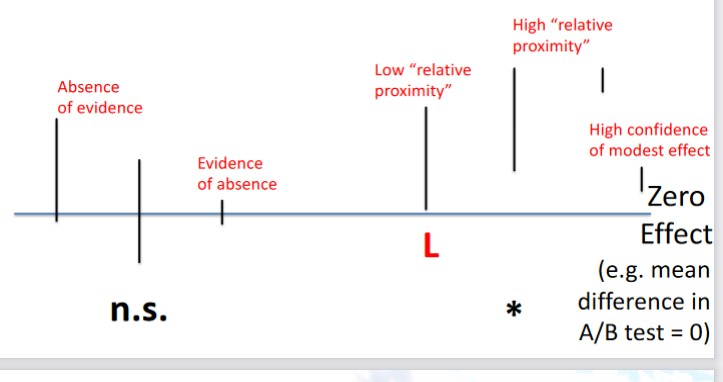
\includegraphics[width=7.5cm]{Final_Review/lecture_5/ci bounds example.jpg}
\item but we could have very narrow confdince intervals around 0, which indicate to us that something is evedince of absance. that is valuable 
\item in a classical null hyptohsis frame work all three first liens map to not signfgent 
\item but sigfegenct or nto sigfgent doe snto give us that much information 
\item the furhterst to the right, is a very small effeect hat we are confidinct in our esimate 
\item we need to get away from chasing good effects and get twoards meausring the effects we have well
\item underpowerd studies have really wide confidicne intervals 
\item the whole idea of the null hyposhiss frmae work is taht we asasusme abssence of evedince so getting a non signfgnet reuslt with low power does not tell us very much, but getting a high power result with out evedince might tell us something 
\item jumping in a circle does not cure covid, if we can show that well we can stop peolpe from neeidng to reaerch that 
\item evedince of absance is valuable
\item  absance of evedince is not valubale
\item so confdince intervlas help us distinugsh difrent types of sigfgnece
\item with great power comes small confidince intervals 
\item pick up at aprox 31 minutes
\end{itemize}


\end{document}
